\chapter{A tervezett architektúra}

A következőkben részletezem a tervezett architektúrát két nézetben: első körben a logikai felépítését mutatom be, majd a fizikai felépítését az AWS-felhőben. A logikai felépítés a követelmények alapján készül függetlenül egy választott platformtól, türközi az alapszintű kommunikációs modelljét az egyes részkomponensei közt a rendszernek, amikre lehet bontani a teljes egészet. Segíti a megértését a mérnök terveinek a megrendelő számára is, aki nem feltétlen teljesen tapasztalt a területen. A fizikai felépítés konkrét szoftverkomponenseket definiál, amelyeket fejleszteni szükségeltetik a rendszer megvalósításához. Inkább a fejlesztőknek szól, akik a rendszer megvalósításáért felelősek.

\section{Logikai felépítés}

A logikai felépítést legjobban a \refstruc{fig:highlevel} tudja jól bemutatni. A rendszer három fő komponenscsoportra bontható a követelmények alapján: a kliensközeli csoportra, a szerveroldali csoportra és az ``orkesztrációs'' csoportra. A kliensközeli csoport szolgálja ki a felhasználókat tartalommal, a szerveroldali csoport kezeli az hagyományos üzleti logikát, ahogy az egy többrétegű webalkalmazás megvalósításánál is megszokott az iparban. Az utolsó csoportot ``orkesztrációs'' csoportnak neveztem el, mivel ez szereli fel a két csoportot tartalommal, kezeli események hatására a videófeldolgozást a háttérben.

Érdekes lehet megfigyelni, hogy az egyes csoportok konkrét megvalósítása akár kicserélhetővé válik, egy-egy csoport mögötti teljes szoftvercsomag könnyen lekapcsolható a másik kettőről, csupán jól definiált és agnosztikus API-okra van szükség.

A kliensközeli csoportban a felhasználók a webalkalmazást saját kliensükre egy erre szolgáló tárolóból kell letöltsék, hasonlóképp érik el a videókat két tárolóból. Ezzel a funkcionális követelmények megvalósulnak az élők elérésére, a VOD-ok elérésére, a weboldalon a videóprojektek UI-jára vonatkozó követelmények. A nem funkcionális követelményekből pedig teljesül a caching komponenssel, hogy a videók gyorsan és megbízhatóan érhetőek el a nézők számára.

A szerveroldali csoportban darabokra szedve tulajdonképpen egy REST API helyezkedik el élőadás-, VOD- és felhasználókezelő komponensekkel közösen. Ez API-átjáró mögé van helyezve, amely a biztonságos kommunikációt tudja biztosítani, a felhasználók autentikációját és autorizációját tudja kezelni együttműködve a felhasználókezelő komponenssel, valamint a kliensnek a megfelelő interakciós lehetőséget tud szolgáltatni. A szerveroldali csoportban a videók feltöltése történik csupán, az egyes entitásokról a változások nyilvántartása kerül még tárolásra.

A szerveroldali csoport események formájában kommunikál az élőadás- és VOD-kezelő az ``orkesztrációs'' csoportban lévő eseménykezelővel. Az orkesztrációs réteg fogja a két csoportot össze, események hatására indíttat konvertálást a konvertáló komponenssel. Ez a komponens tölti fel a videókat a kliensközeli csoport felé, tart összeköttetést a live streaming külső forrásával.

\begin{figure}[ht]
	\centering
	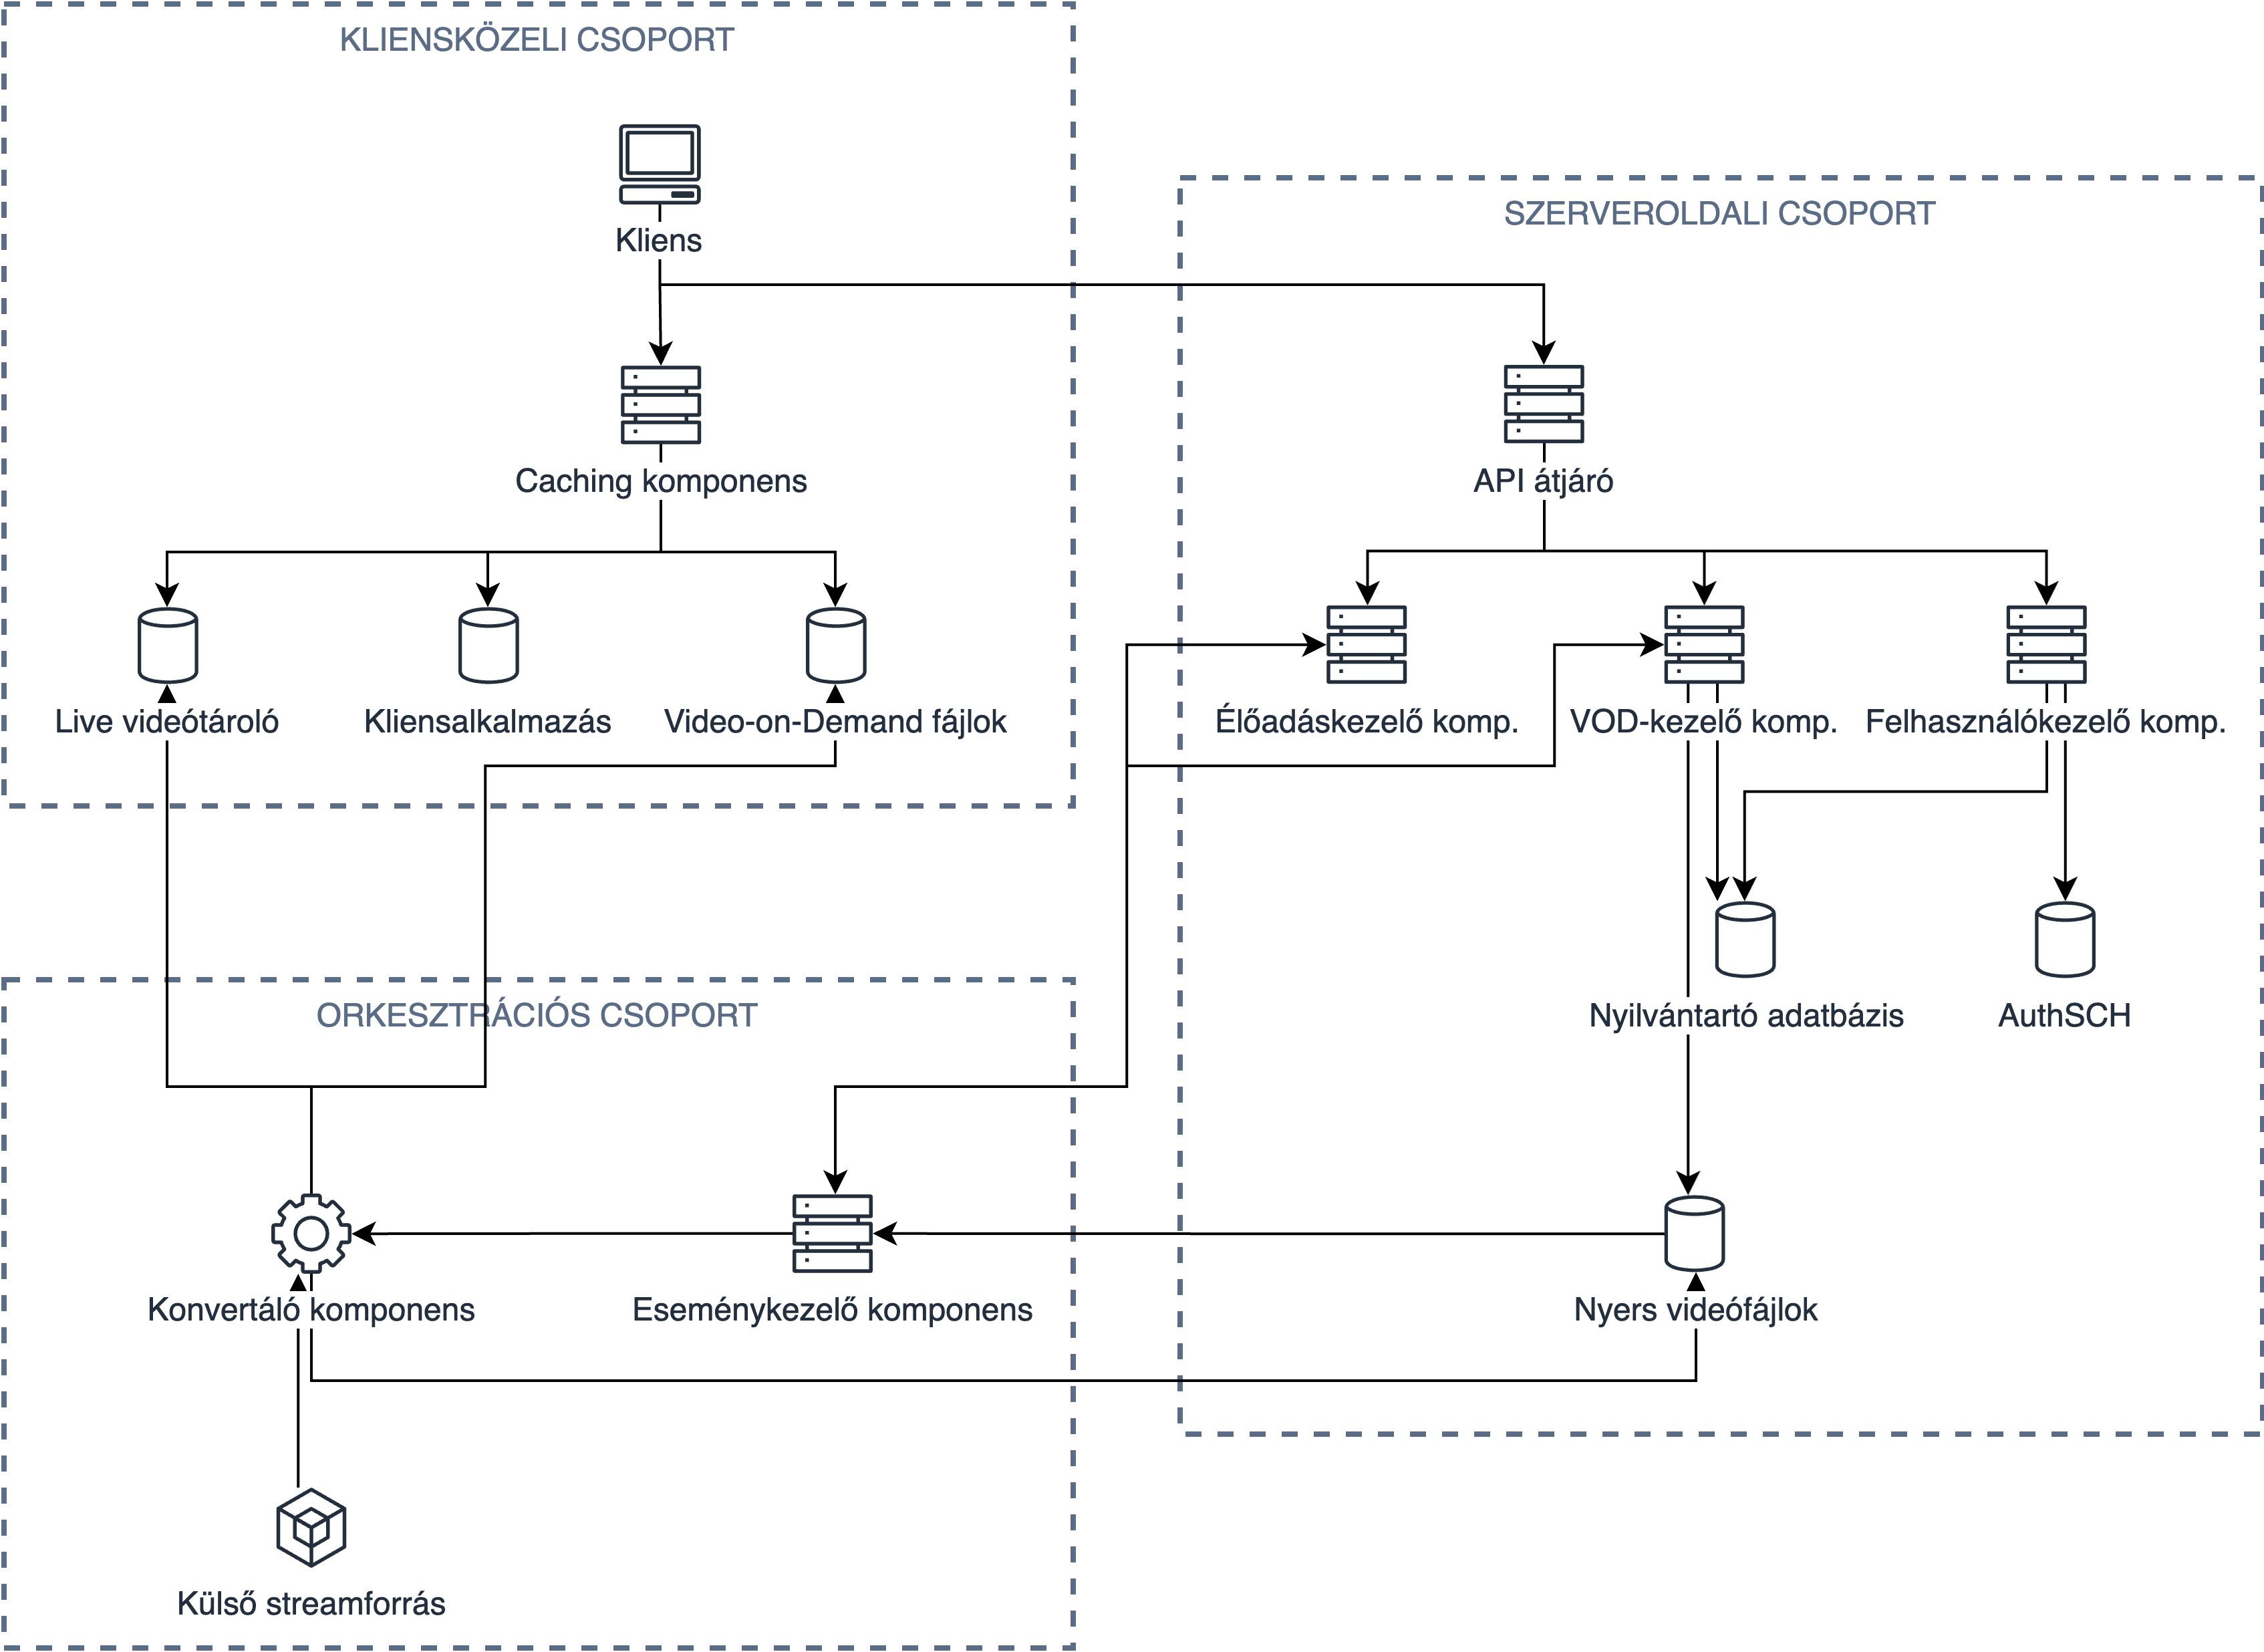
\includegraphics[width=140mm, keepaspectratio]{figures/dipterv_highlevel.png}
	\caption{Logikai felépítés a követelmények alapján.}
	\label{fig:highlevel}
\end{figure}

Megjegyzés: az itt feltüntetett komponensek élőadás-, VOD- és felhasználókezelő moduljai a későbbiekben a konkrét szoftverarchitektúrában monolit struktúrában egy közös szerveralkalmazásba kerültek bele, azon belül kerültek modularizálásra az üzleti logikában.

A korábbi \ref{streamref}. alfejezetben megismert protokollok közül a tervezés során az egyszerű implementáció és a jól támogatottság szempontjából a HTTP Live Streaming (HLS) protokollt választottam a VOD és live streaming fogadó oldalán. Az élő közvetítéshez a Real-Time Messaging Protocol (RTMP) protokollt választottam, ehhez az OBS Studiót használtam a felstreameléshez.

\subsection{Összehasonlítás egy hasonló rendszerrel}

A tervek igazolásához segítségül kerestem az interneten nyílt forráskódú hasonló megoldásokat is. Megtaláltam a Technische Universität München (TUM) egy hallgatói csoportja, a TUM-Dev által fejlesztett az egyetemen is használt VoD és live streaming szolgáltatását, a GoCastot\footnote{\url{https://github.com/TUM-Dev/gocast}}. Ez a rendszer önállóan hosztolható szoftvereket komponál össze, nem felhőnatív. A rendszerben hasonló absztrakt terveket lehet megfigyelni az én megoldásaimhoz (\refstruc{fig:gocast}), ugyanígy HLS-sel szolgálják ki a tartalmakat (lásd \emph{TUM-Live Edge} példányok), viszont a live streamingre saját több portos workereket alkalmaznak (lásd \emph{TUM-Live-Worker} példányok), lehetőség ad viszont saját streamerből RTMP-n keresztül feltölteni élő közvetítést, ahogy én is megvalósítom a saját megoldásomban. Külön mikroszolgáltatás biztosítja a live és VOD streamingen kívüli funkcionalitásokat, a TUM-Live. Ez a megoldás nem teszi lehetővé, hogy a rendszeren kívül készült videót lehessen feltölteni és VOD-ként elérhetővé tenni rajta keresztül.

\begin{figure}[ht]
	\centering
	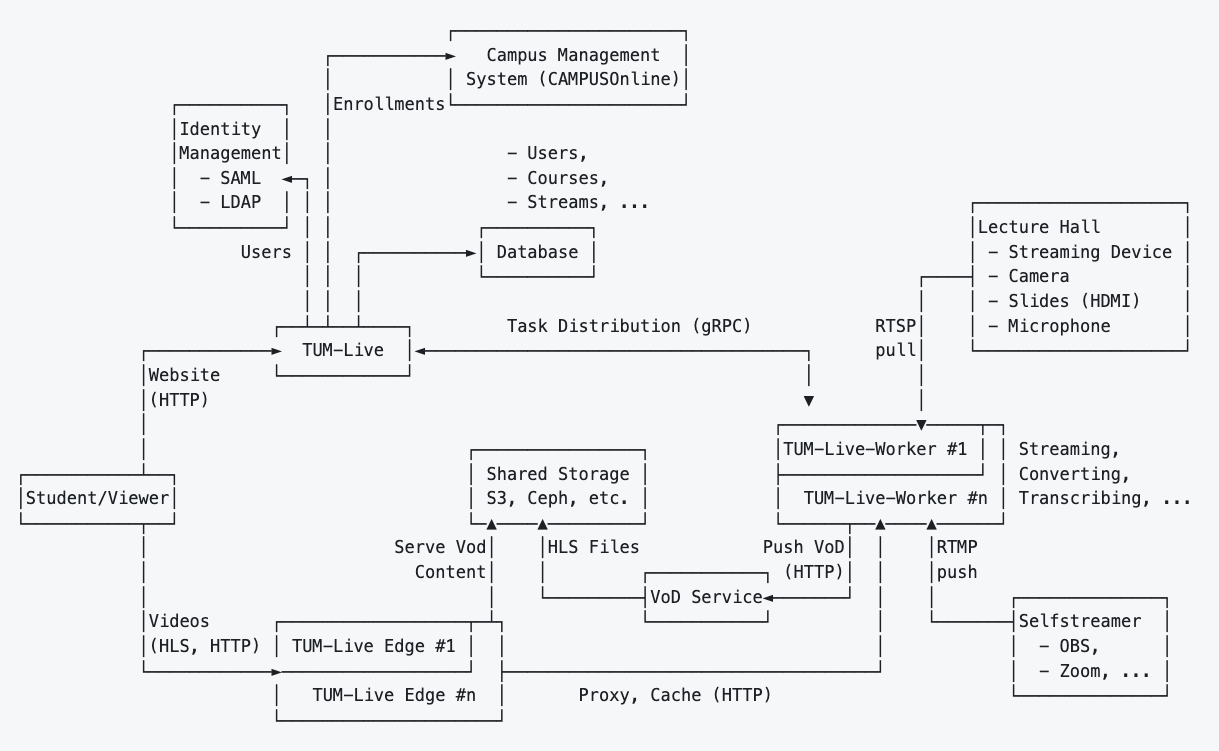
\includegraphics[width=140mm, keepaspectratio]{figures/gocast.png}
	\caption{A GoCast architektúrája a dokumentációból.}
	\label{fig:gocast}
\end{figure}

\section{Fizikai felépítés AWS-re specializáltan}

A rendszert az átlátható kezelés érdekében az AWS-felhőben egy teljesen erre külön készített AWS-fiókba helyeztem, így terveztem meg az architektúrát is. A rendszer egyszerűsített fizikai felülnézetét az AWS-fiókban, az AWS-erőforrások összeköttetését jól összefoglalja az \refstruc{fig:architect}.

Az ábrát olvasva látható, hogy egészen jól elkülönülhetnek ebben a nézetben is csoportokra az egyes erőforrások. A kliensközeli csoportot a CloudFront CDN szolgálja ki, ennek a disztribúciónak adtam domainnevet, így használatba került egy stream.trisz.hu domain alatti Amazon Route53-zóna is, illetve egy SSL-tanúsítvány is hozzáadásra került. A védelmezésre egy AWS Web Application Firewall web Access Control List -- röviden: egy WAF web ACL -- is bekerült a disztribúció elé. Ezen szolgáltatások az edge szerverfarmokon működnek, az AWS ehhez azt írja elő, hogy az erőforrásokat a ``us-east-1'', azaz az észak-virginiai régióban kell elhelyezni.

A disztribúció után jönnek egy új rétegben először egy ALB-példány, ez és a mögötte lakó erőforrások az ``eu-central-1'' (frankfurti) régión belül is egy saját hálózatba, azaz AWS VPC-be kerültek. Ezenkívül videók S3-vödrét, a React alkalmazás vödrét és a live csatornát mind külön originként tettem a disztribúció mögé, külön-külön útvonalak mintázatokra illeszkedve.

A RTMP-alapú live stream fogadását OBS Studióból a MediaLive kezeli, ami a MediaPackage segítségével továbbítja egy csatornán a tartalmat. A VOD-tartalmakat a MediaConvert konvertálja HLS-adatfolyamba illeszthető formátumba, a kimenetét pedig a S3-vödörbe helyezi. A szerveralkalmazás egy Node.js alapú web app a terveim alapján, amely NestJS keretrendszerrel kerül kialakításra, Dockerrel konténerizálom és az ECS-be telepítem, azzal menedzselem életciklusát; az ECR-be kerülnek a konténer képei. Az adatbázis egy PostgreSQL példánnyal kerül megvalósításra, amelyet az RDS szolgáltatásban helyezek el menedzselésre.

Az orkesztrációs eseményekre Lambda-függvények reagálnak, az eseményeket központilag az EventBridge hallgatja le szabályokkal és kötteti össze a megfelelő Lambda függvényekkel. Felhasználásra kerülnek a biztonságos kezelésre IAM-szerepkörök, monitorozásra és naplózásra a CloudWatch, illetve az érzékeny paraméterek tárolására az AWS Secrets Manager.

A kódbázis GitHubon kerül verziókezelésre, ott a CI/CD-folyamatokat GitHub Actions segítségével automatizálom a szerveralkalmazás élesítésére, a React-alkalmazás statikus fájljainak feltöltésére. A Terraform segítségével az infrastruktúrát kód formájában kezelem, a Terragrunt -- amely egy Terraform-kódkezelést segítő kiegészítő eszköz -- pedig a Terraform-modulokat kezeli, hogy a kódbázis ne legyen túl bonyolult.

\vspace{2cm} % remove, if unnecessary

\begin{figure}[!ht]
	\centering
	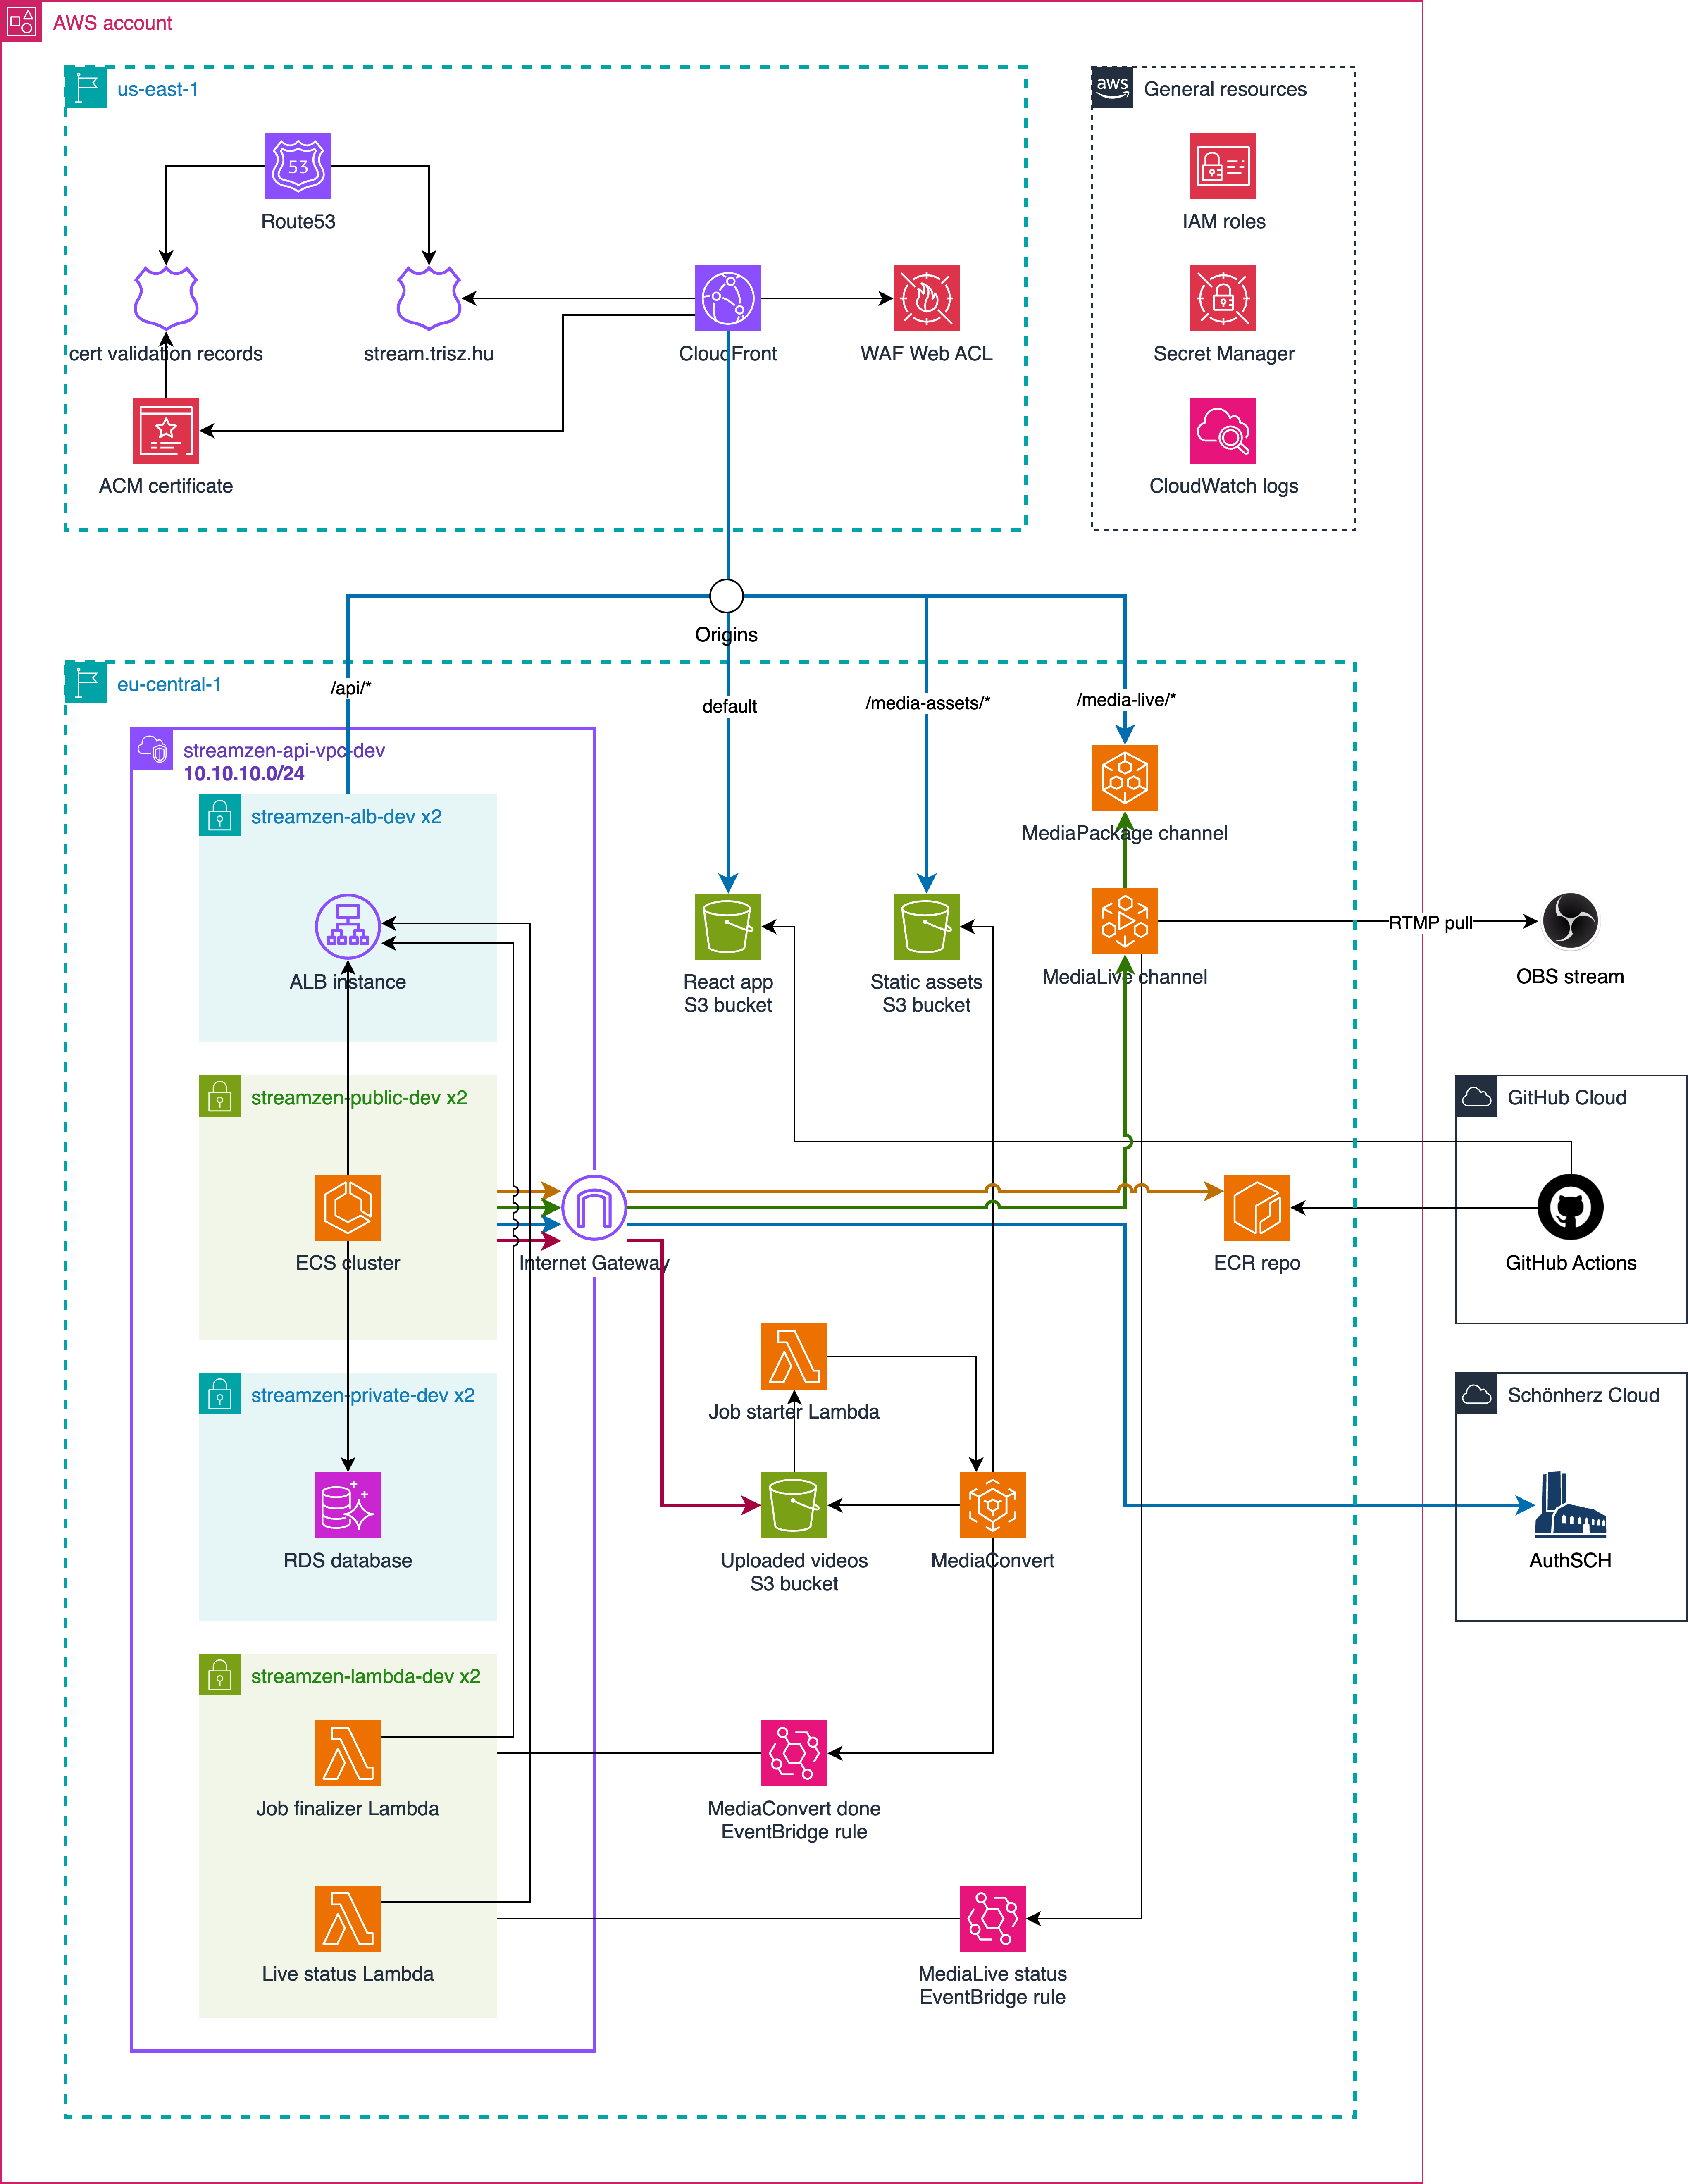
\includegraphics[width=160mm, keepaspectratio]{figures/dipterv_architect.png}
	\caption{Az AWS-fiók erőforrásainak logikai kapcsolata.}
	\label{fig:architect}
\end{figure}

\vspace{2cm} % remove, if unnecessary

\subsection{Video-on-Demand kiszolgálás folyamata}

Vizsgáljuk meg közelebbről a VOD-tartalom kiszolgálásának folyamatát az AWS-felhőben. A \refstruc{fig:vod1} mutatja be a VOD-tartalom feltöltésének folyamatát, ahol a szerveralkalmazás a nyers videót buffer formájában fogadja HTTPS-en keresztül a böngészőből. A webszerver az S3-vödörbe helyezi, illetve lenyugtázza az adatbázisban, hogy a konvertálási folyamat ezzel elindult. A folyamatot a felhasználói felületen a felhasználók követhetik, ahol a folyamat állapotát mutatja a szerveralkalmazás.

\begin{figure}[ht]
	\centering
	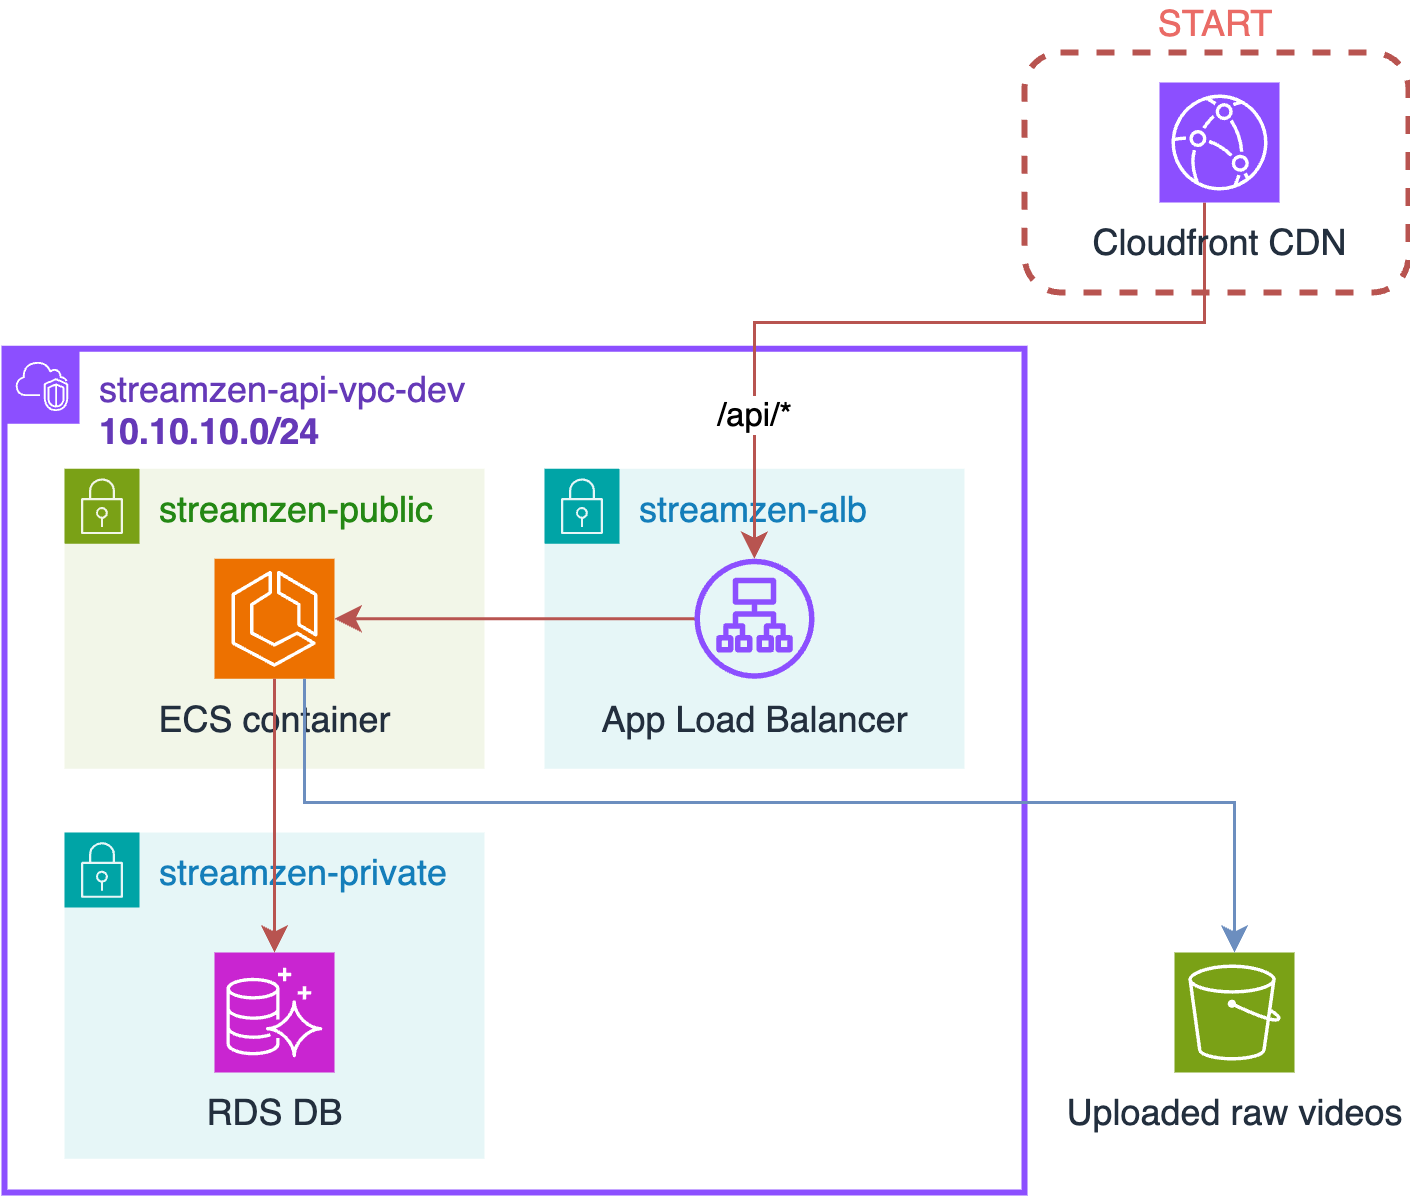
\includegraphics[height=60mm, keepaspectratio]{figures/dipterv_vod1.png}
	\caption{Folyamatábra a nyers videó feltöltéséről.}
	\label{fig:vod1}
\end{figure}

A \refstruc{fig:vod2} mutatja be, hogy fut le a feltöltés utáni folyamat. Egy konvertálási jobot indító Lambda-függvény feliratkozik a feltöltött videókat tároló S3-vödörre, amely a feltöltés után felkonfigurál egy jobot a MediaConvert számára, megadja a forrásfájlt és az S3-vödröt, ahova majd a job után kell kerüljön a HLS-kompatibilis fájlcsomag. Egy másik Lambda-függvény, amely a MediaConvert job állapotváltozásaira van feliratkozva, a folyamat végén értesíti a webszervert az ALB-n keresztül, hogy nyugtázza a folyamat jelenlegi státuszát.

\begin{figure}[!ht]
	\centering
	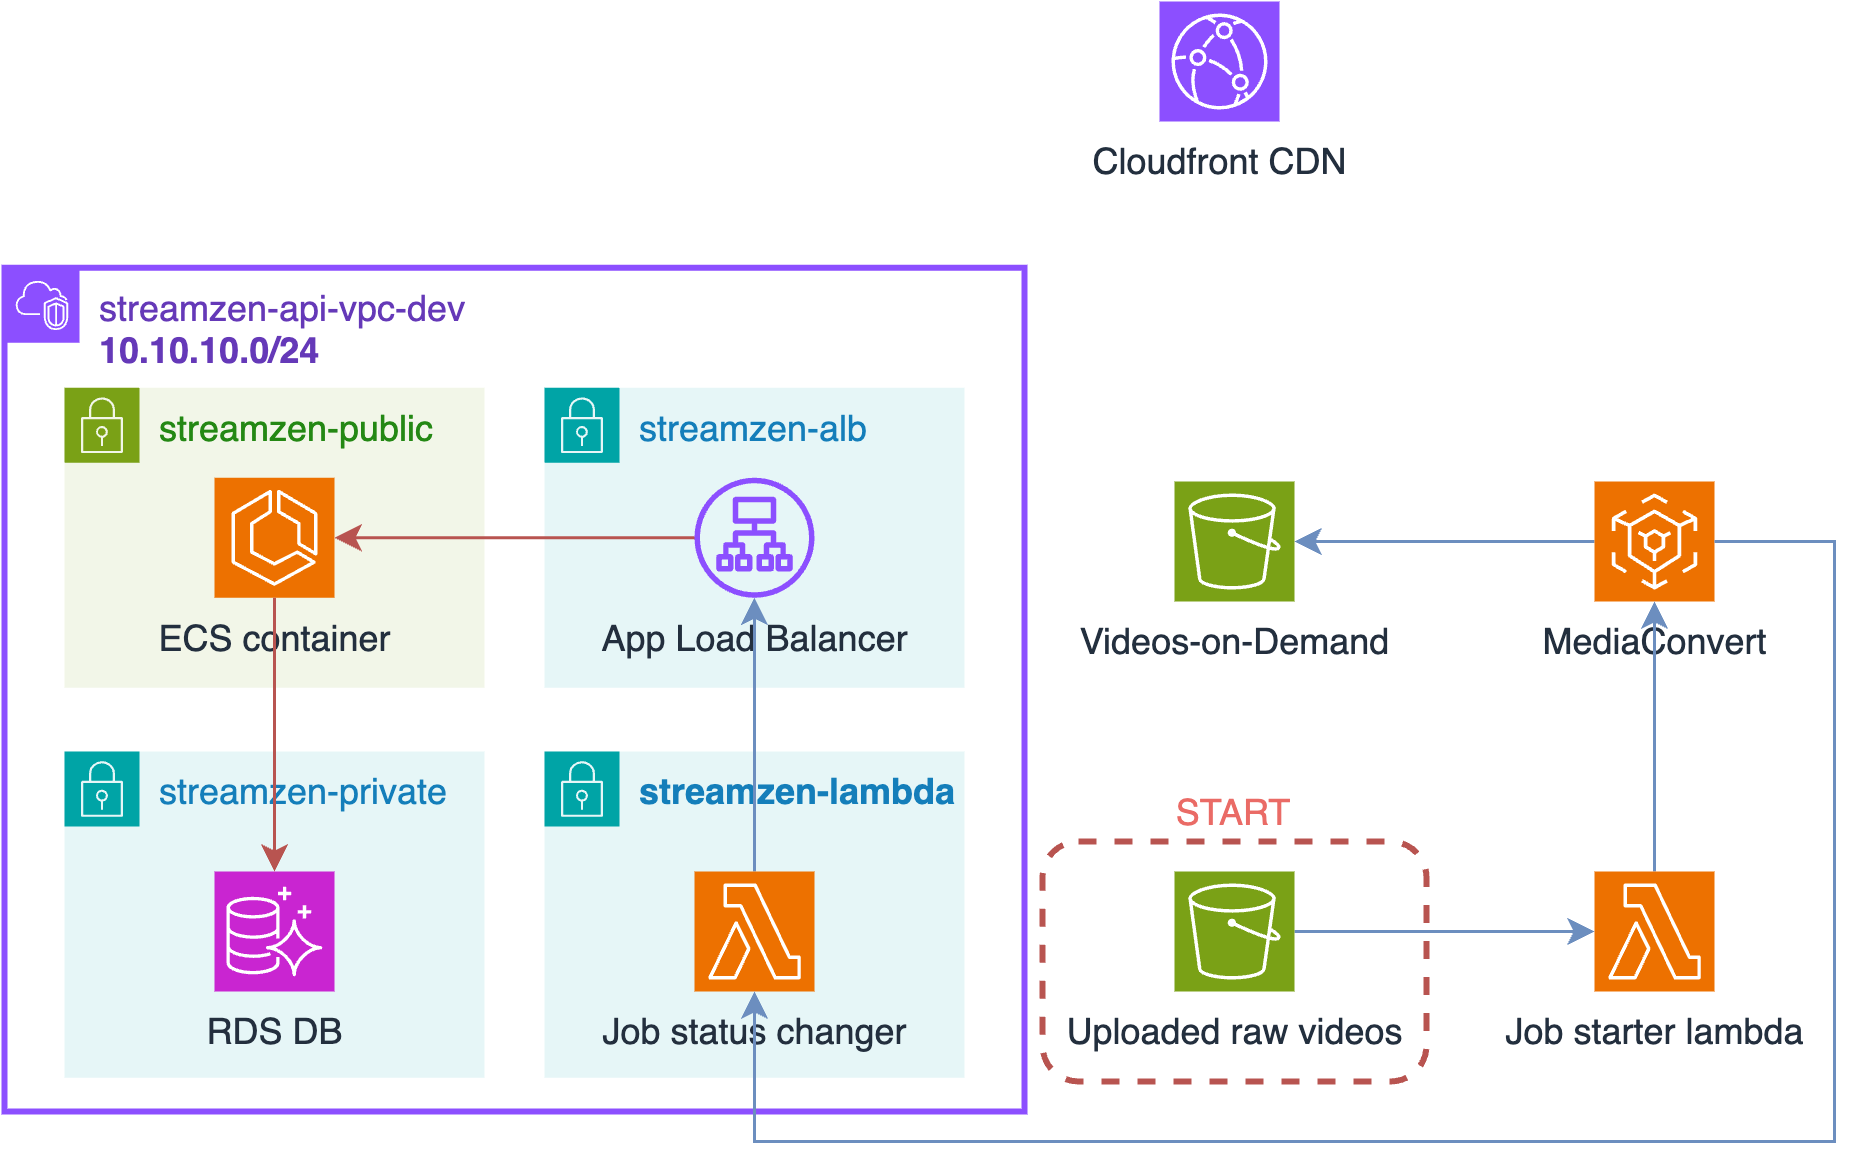
\includegraphics[height=60mm, keepaspectratio]{figures/dipterv_vod2.png}
	\caption{Folyamatábra a feltöltés utáni videófeldolgozásról.}
	\label{fig:vod2}
\end{figure}

A \refstruc{fig:vod3} fejti ki egy részről, hogy hogy értesül az adminisztrátor a videó feldolgozottságának állapotáról az API-n keresztül, illetve a UI-n értesülés után mi történik, ha meg is nyitja a már streamelhető videót, amely a CloudFront disztribúció Video-on-Demand S3-alapú originjén keresztül érhető el.

\begin{figure}[!ht]
	\centering
	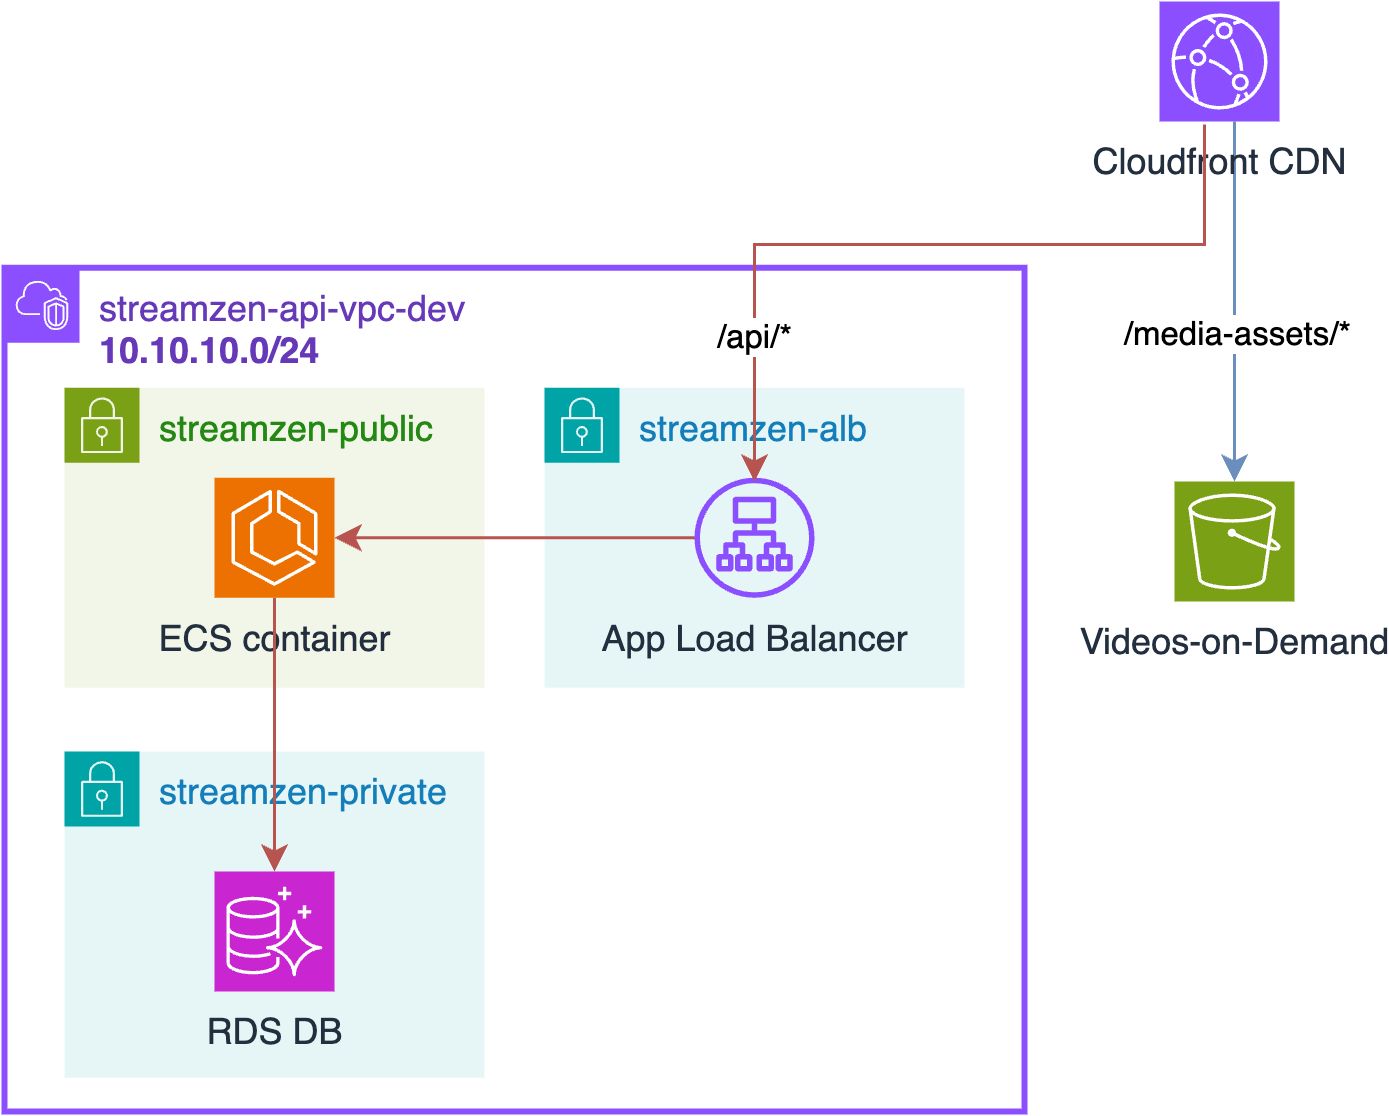
\includegraphics[height=60mm, keepaspectratio]{figures/dipterv_vod3.png}
	\caption{Folyamatábra a VOD-tartalom lejátszásáról.}
	\label{fig:vod3}
\end{figure}

\subsection{Live streaming folyamata}

A live streaming indítását mutatja be a \refstruc{fig:live1}. Az adminisztrátor a stúdióban gombnyomásra megnyitja API-n keresztül a live streamet, amellyel a MediaLive szolgáltatásban a csatorna is elindul, aktívan húzza RTMP-n keresztül a felcsatlakoztatott forrásból a videóanyagot.

\begin{figure}[ht]
	\centering
	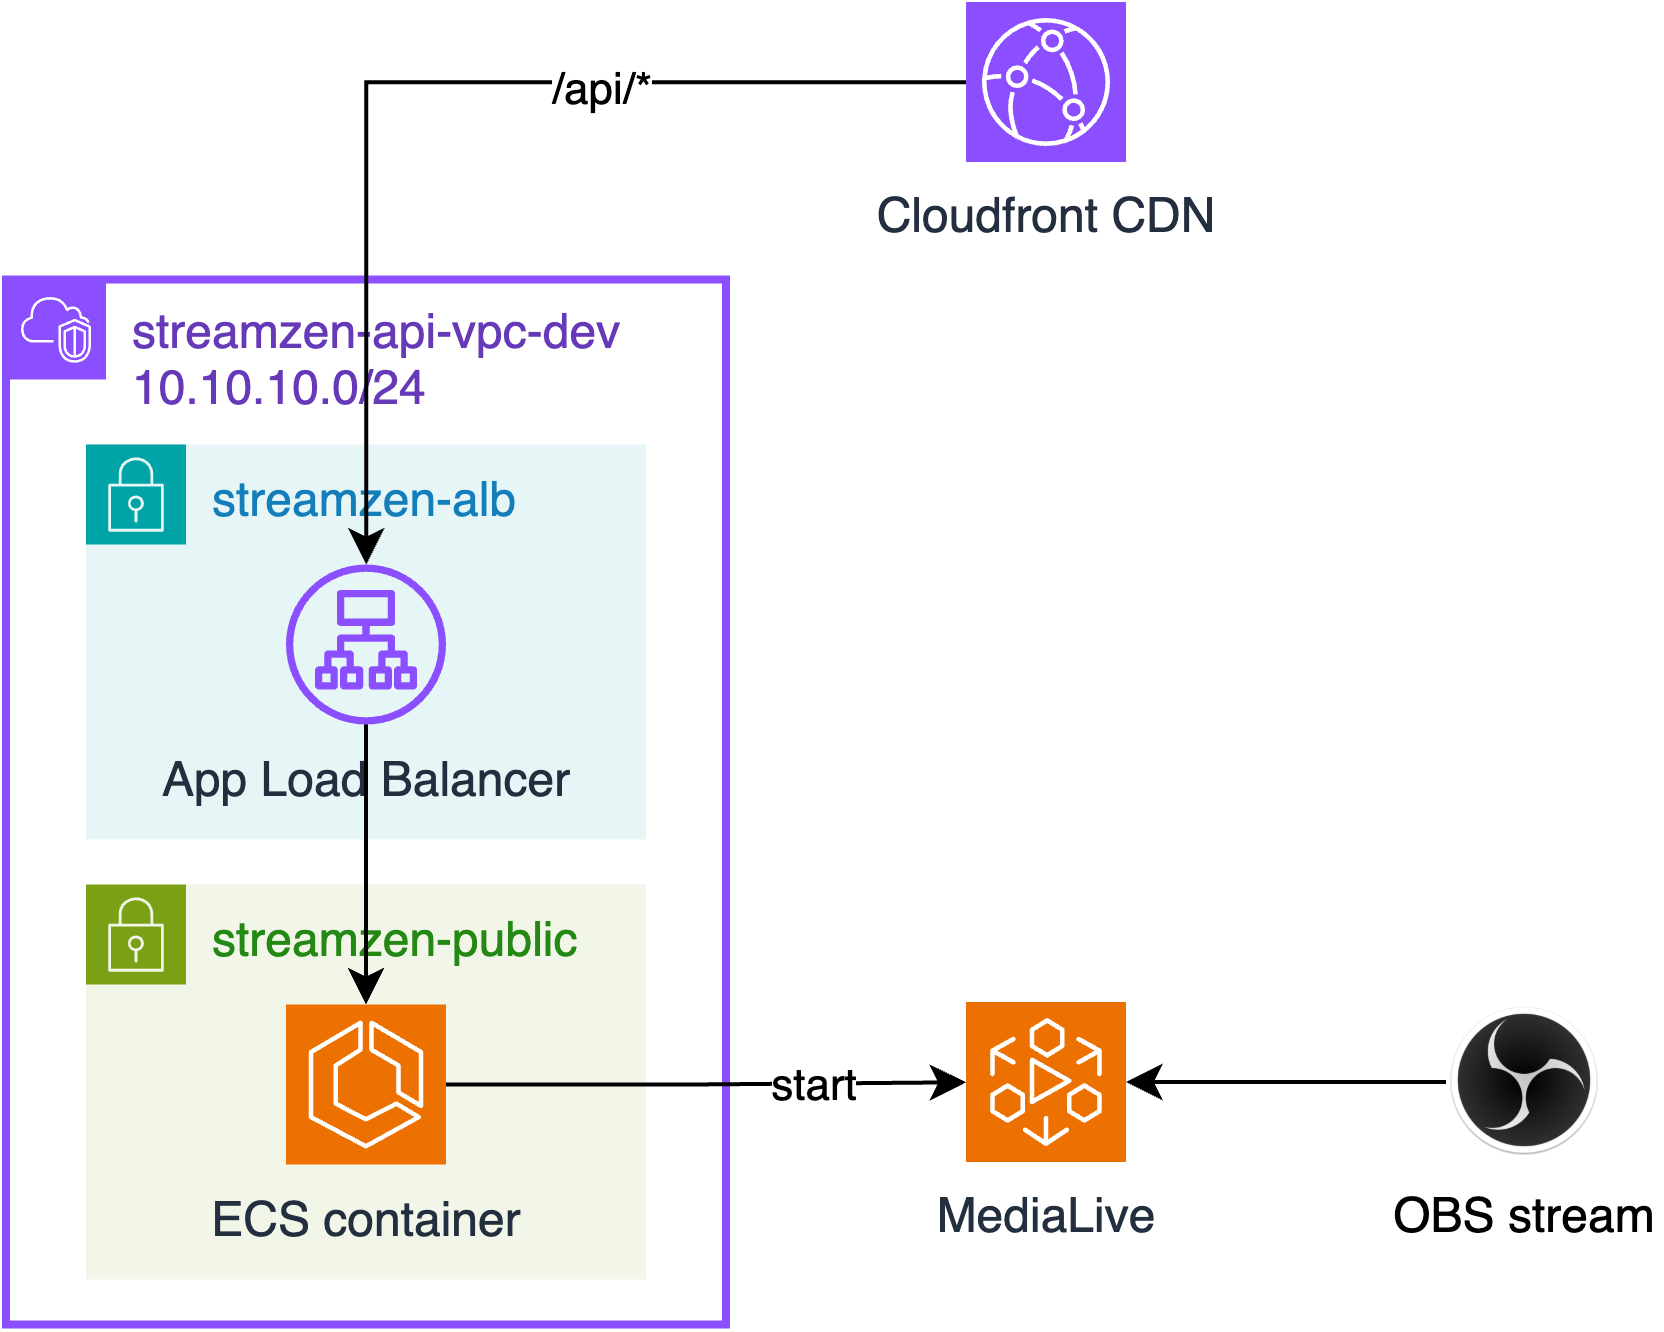
\includegraphics[height=60mm, keepaspectratio]{figures/dipterv_live1.png}
	\caption{Folyamatábra a live stream indításáról.}
	\label{fig:live1}
\end{figure}

\vspace{2cm} % remove, if unnecessary

A \refstruc{fig:live2} pedig bemutatja, miután a live stream elindult, a MediaPackage csatorna húzza át a konvertált videót a CloudFront disztribúció elé, így ezen az originjén keresztül lesz elérhető a Cloudfront disztribúciónak a felhasználók számára, akik a webalkalmazásban a megfelelő útvonalon érik el a live streamet.

\begin{figure}[ht]
	\centering
	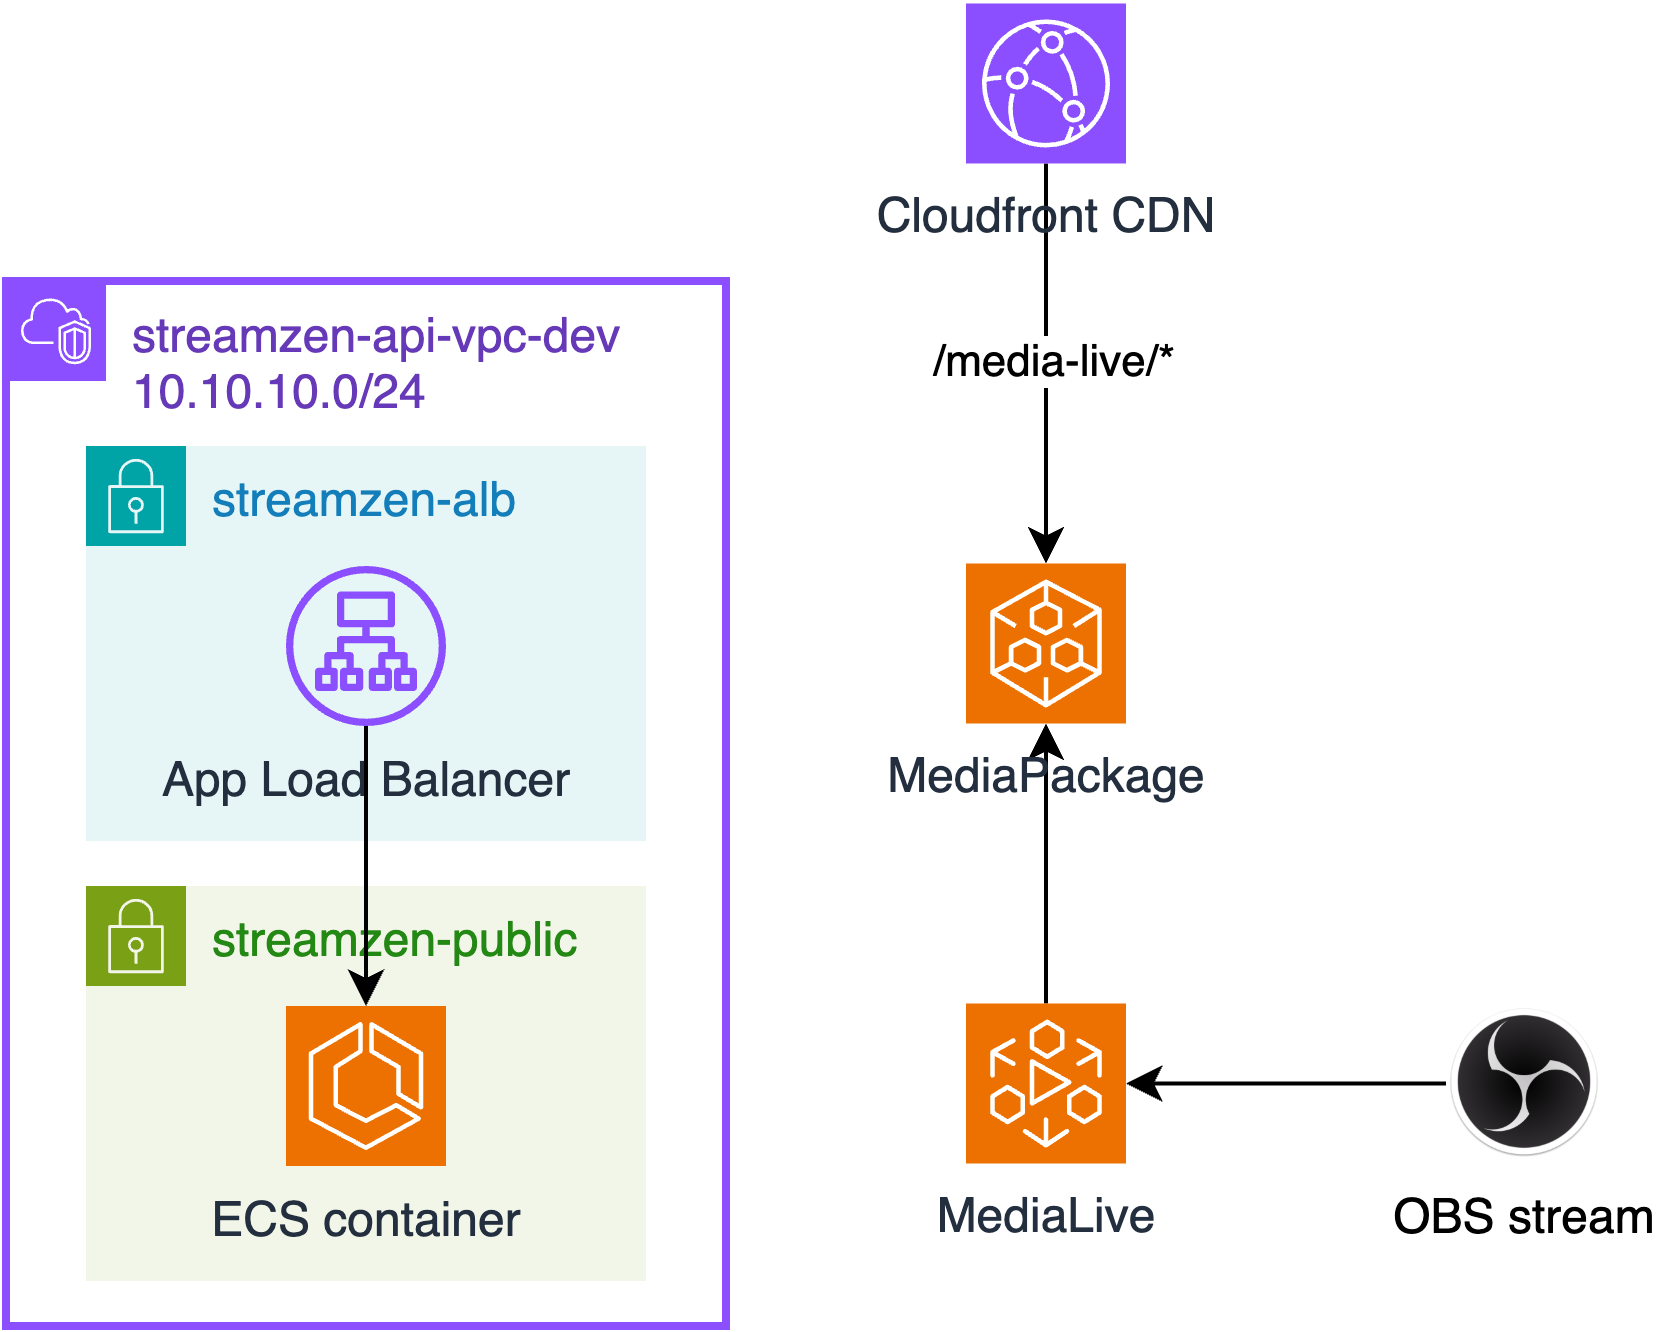
\includegraphics[height=60mm, keepaspectratio]{figures/dipterv_live2.png}
	\caption{Folyamatábra a live streamre való kapcsolódásról.}
	\label{fig:live2}
\end{figure}

\section{Konfigurációmenedzsment}\label{sec:config}

Nagyobb rendszerek tervezése igényli, hogy megfelelő Konfigurációmenedzsmentet teremtsen köré a tervezőmérnök, hogy a rendszer könnyen karbantartható legyen. A Terraform lehetővé teszi az infrastruktúra építését és az annak felkonfigurálását kód formájában, a kódban való élesítések nyomán friss és dokumentált marad az állapota is ezeknek.

Egyetlen környezetet terveztem kialakítani, egy \emph{development}, azaz fejlesztési környezetet, a Terraform modulokat egy befoglaló Terragrunt gyökérmodulba szerveztem, a \verb|streamzen-core| mappába. Az erőforrásokat igyekeztem olyan módon elnevezni, hogy azok tartalmazzák a \verb|streamzen| prefixet és a környezet nevét, például \verb|dev| is tartalmazzák, hogy könnyen lehessen azonosítani őket a későbbiekben. Az erőforrások alapvetően az ``eu-central-1'' régióban helyezkedtem el, a globális erőforrások kivételével.

Terraformban menedzselt infrastruktúra tipikus életciklusa áll a kódból származó tervek előállításából (plan), annak manuális átolvasásából, majd pedig a változtatások aktiválásából (apply). Az automatizálás érdekében GitHub Action munkafolyamatokba terveztem szervezni a Terraform tervek előnézetének generálását -- amely a \verb|terraform plan| parancs kiadasával kezdeményezhető -- , ami minden Pull Request (PR) UI-ján kommentként kerül hozzáadásra a PR-hez, viszont a tervek élesítését (erre használt parancs a \verb|terraform apply|) saját kézzel a saját parancssoromból terveztem megtenni, tekintettel arra, hogy csupán egyedül dolgoztam a kódbázissal.

Hogy az AWS-fiók erőforrásaihoz hozzáférést kaphasson a munkafolyamat is, a GitHub Action munkafolyamata számára OpenID Connect (OIDC) felállításával terveztem az erre szánt AWS-szerepkör felvételét megvalósítani (\refstruc{fig:githuboidc}\footnote{A kép forrása: \url{https://mahendranp.medium.com/configure-github-openid-connect-oidc-provider-in-aws-b7af1bca97dd}}). \cite{githuboidc}

\begin{figure}[ht]
	\centering
	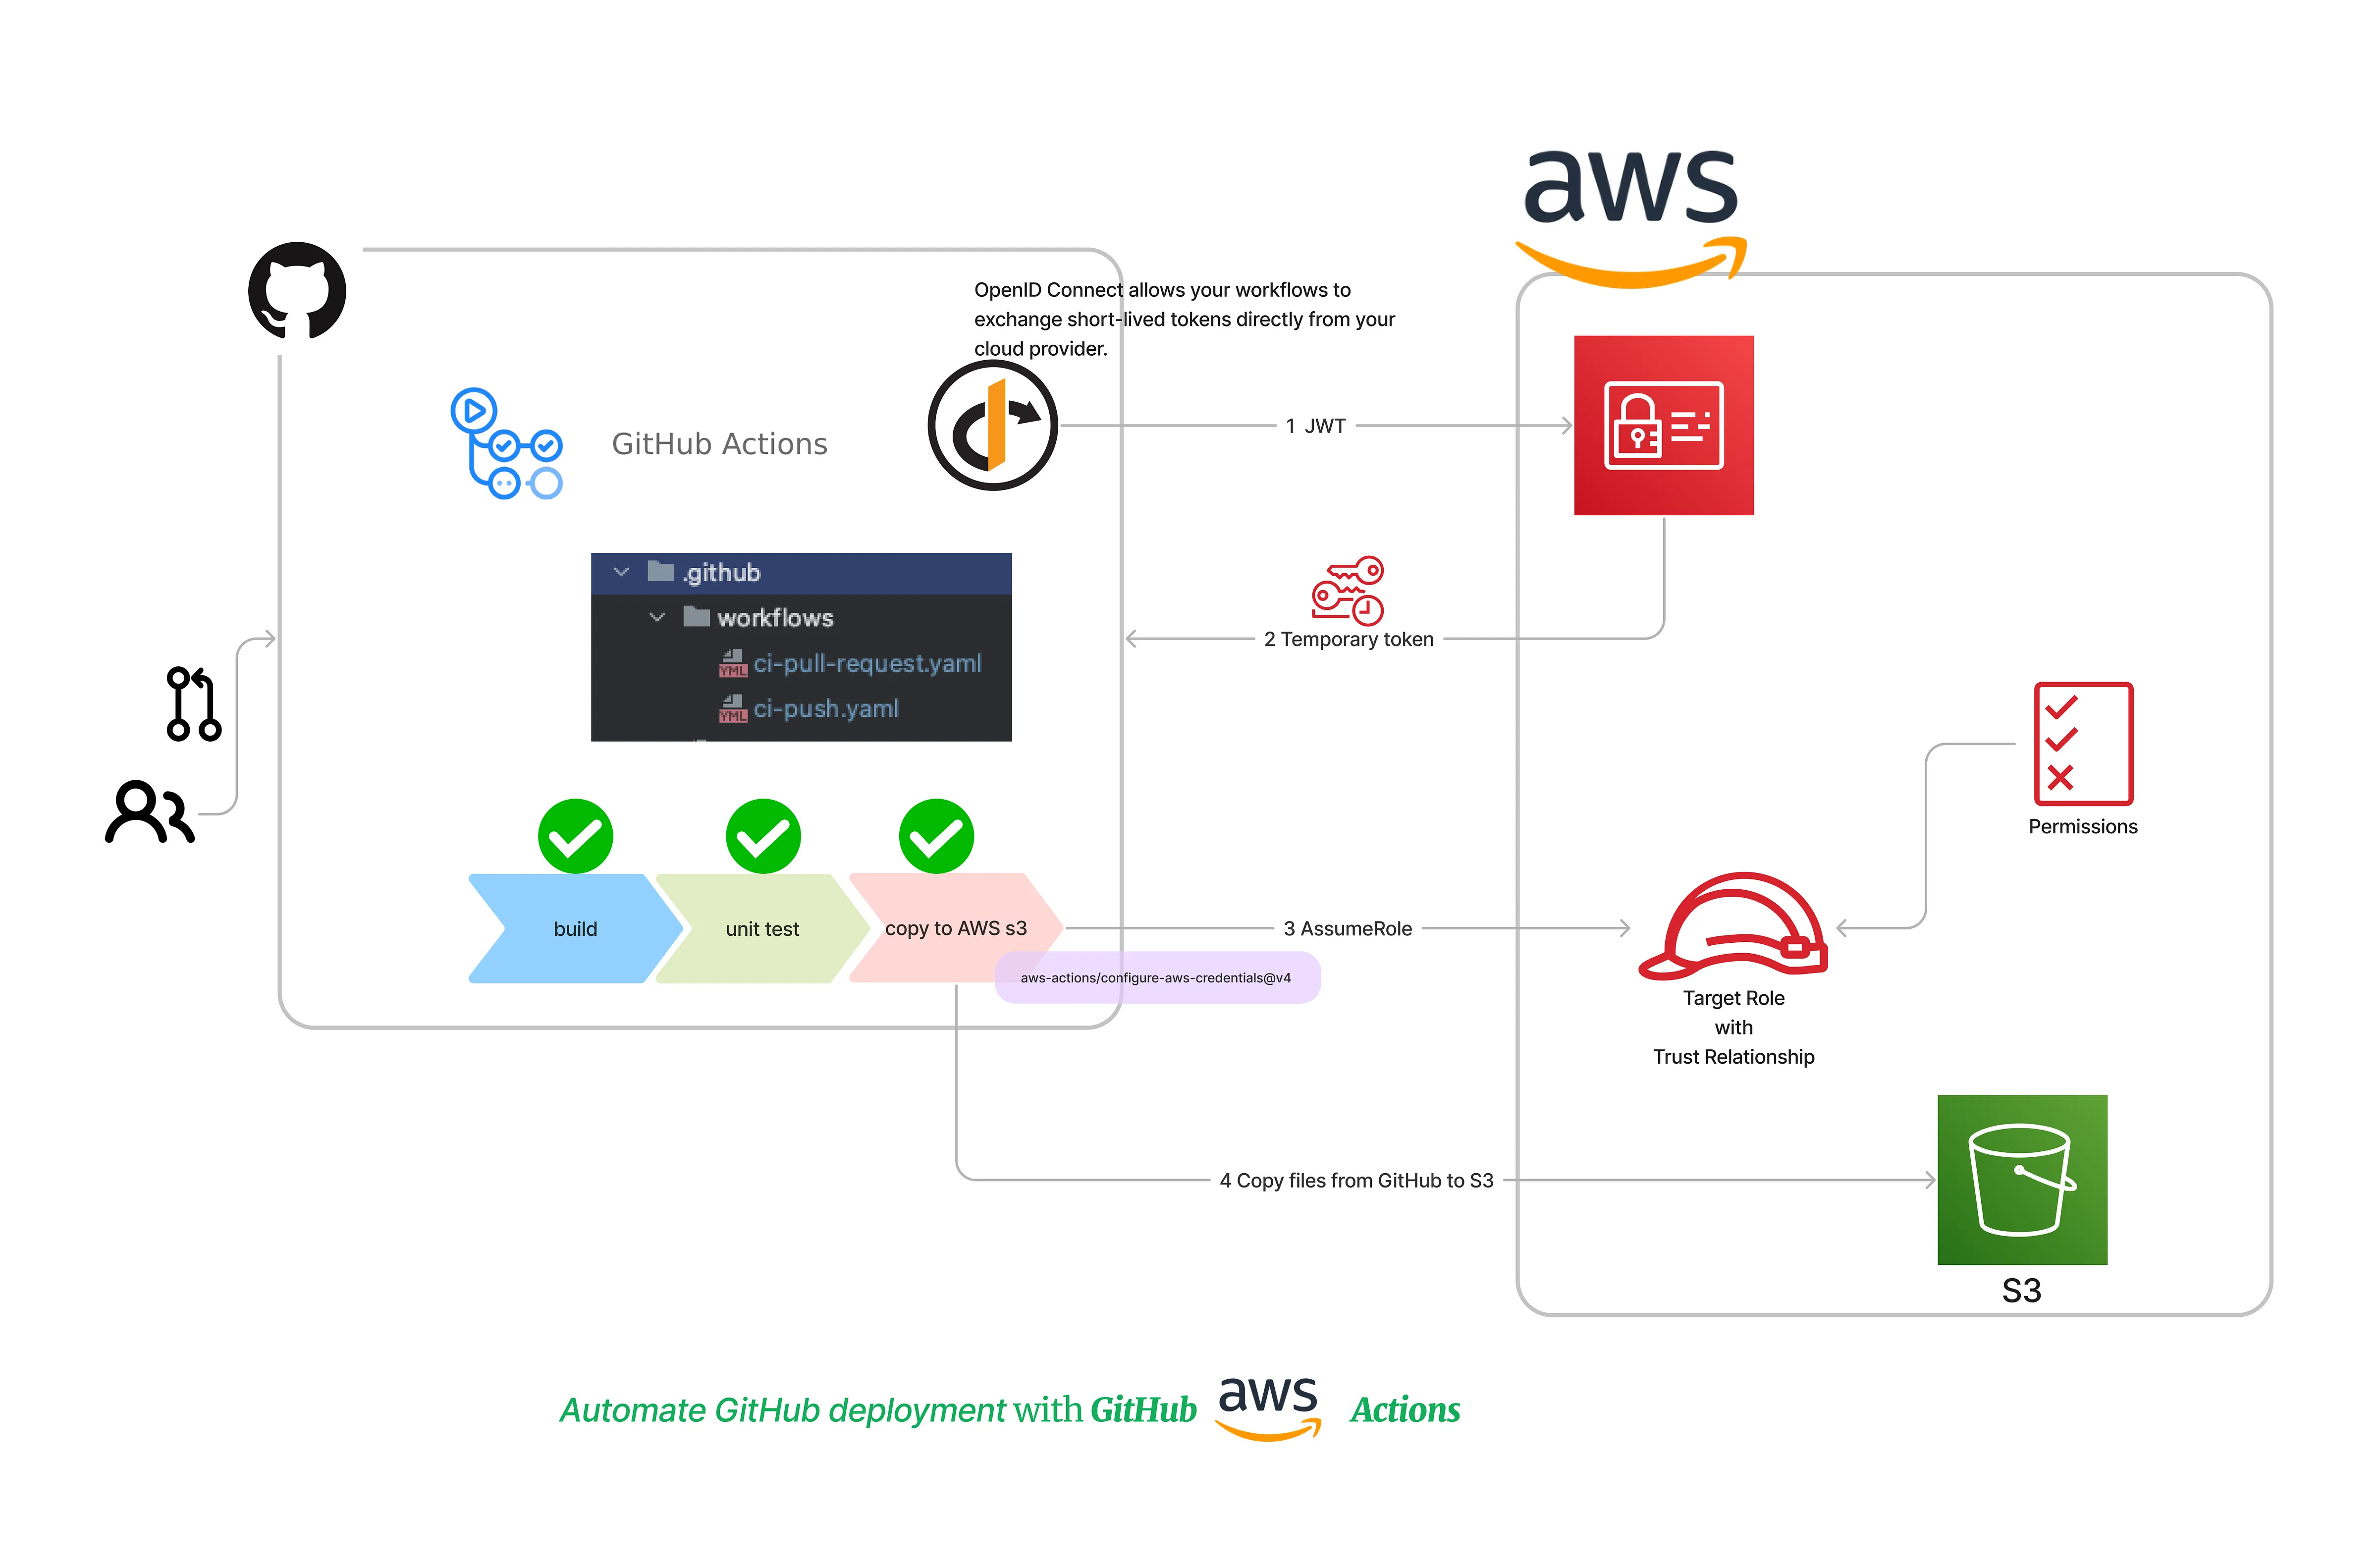
\includegraphics[width=150mm, keepaspectratio]{figures/githuboidc.png}
	\caption{Workflow autorizálása AWS-szerepkörre OIDC-val.}
	\label{fig:githuboidc}
\end{figure}

A konfigurációmenedzsment részeként még a változtatások hibamentes élesítése érdekében statikus ellenőrzést terveztem bevezetni hasonlóan GitHub Action munkafolyamatokból a React-kód és a szerveralkalmazás Node.js-kódjára is.

A szerveralkalmazás egységként való kezelése érdekében és a könnyű telepíthetőségért -- ahogy ezt a nem funkcionális követelmények is megkívánták -- konténerizálni terveztem a Node.js-szerveralkalmazást Docker-konténerbe való komponálással, a buildelési folyamatot Dockerfile-lal kívántam megvalósítani hozzá. GitHub Action került alkalmazásra az buildelt Docker-kép ECR-be való automatizált feltöltésére (\refstruc{fig:ecr}), a React-kód buildelésére és S3-vödörbe való feltöltésére.

\begin{figure}[ht]
	\centering
	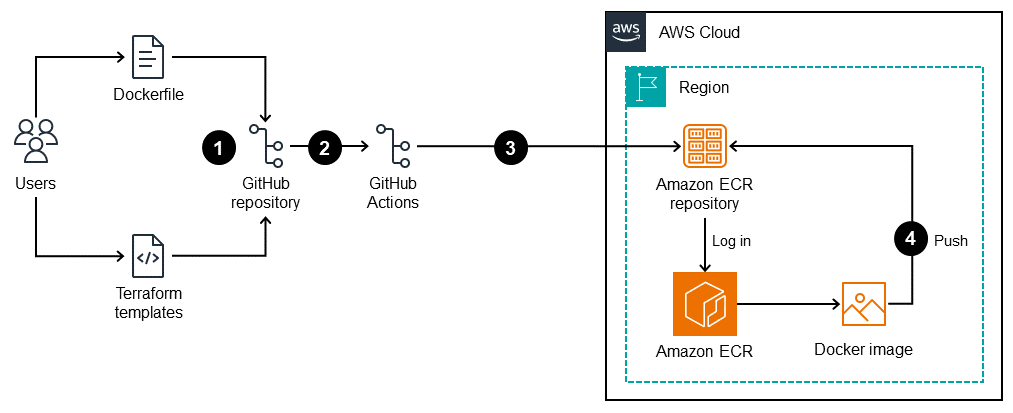
\includegraphics[width=140mm, keepaspectratio]{figures/ecr.png}
	\caption{Folyamatábra a Docker-kép ECR-be feltöltéséről.}
	\label{fig:ecr}
\end{figure}

\section{A projekt felépítése}

A projekt egészét egy közös GitHub-repositoryba terveztem kivitelezni, tehát ``monorepo'' jelleggel. A TypeScript-alapú projektekre bő eszköztárat és könnyű kezelést biztosít a Visual Studio Code (röviden VSCode\footnote{\url{https://code.visualstudio.com/}}) szövegszerkesztő, amelyben a projekt könnyű átláthatóságára pedig egy VSCode-os (\verb|streamzen.code-workspace| fájlnévvel) munkatér-konfigurációt alakítottam ki 5 fő mappából álló struktúrával: \verb|client|, \verb|server|, \verb|infra|, \verb|infra-bootstrap| és \verb|.github| alatt.

A \verb|client| mappában a React-alprojekt található, a \verb|server| mappában a szerveralkalmazás Node.js-alprojektje, az \verb|infra| mappában a Terragrunt-konfiguráció, az \verb|infra-bootstrap| mappában az egyszer aktiválandó Terraform-konfiguráció található (ez állította fel az S3-vödröt a Terraform-állapot tárolására és a CI/CD-csővezeték kapcsolódását OIDC-n keresztül az AWS-fiókba), a \verb|.github| mappában pedig a GitHub Action-munkafolyamatok találhatóak a csővezetékre.
